\documentclass[11pt,letterpaper]{article}
\usepackage[utf8]{inputenc}

%----- Configuración del estilo del documento------%
\usepackage{epsfig,graphicx}
\usepackage[left=2cm,right=2cm,top=1.8cm,bottom=2.3cm]{geometry}
\usepackage{fancyhdr}
\usepackage{lastpage}
\usepackage{url}
\pagestyle{fancy}
\fancyhf{}
\rfoot{\textit{Página \thepage \hspace{1pt} de \pageref{LastPage}}}


%------ Paquetes matemáticos básicos --------%
\usepackage{amsmath}
\usepackage{amssymb}
\usepackage{amsthm}

\usepackage[spanish]{babel}
\usepackage{graphicx}
\usepackage{hyperref}

\usepackage{tabularx}
\usepackage{xcolor}
\usepackage[table]{xcolor}
\usepackage{colortbl}
\usepackage{array, multirow, multicol, tabularx}
\usepackage{tcolorbox}
\newtheorem{theorem}{Theorem}[section]
\newtheorem{corollary}{Corollary}[theorem]
\newtheorem{lemma}[theorem]{Lemma}

%------si-------%
\definecolor{B}{HTML}{FFFFFF}
\definecolor{G}{HTML}{5e5e5e}
\definecolor{R2}{HTML}{d53d40}
\definecolor{A2}{HTML}{034190}
\definecolor{V2}{HTML}{7faa50}
\newcommand{\R}{\mathbb{R}}
\newcommand{\C}{\mathcal{C}}
\newcommand{\Z}{\mathbb{Z}}
\newcommand{\Q}{\mathbb{Q}}
\newcommand{\N}{\mathbb{N}}
\newcommand{\Li}{\mathfrak{L}}
\renewcommand{\theenumi}{\Roman{enumi}}
\renewcommand{\labelenumi}{{\theenumi}.}

\begin{document}
\makeatletter
        \renewenvironment{proof}[1][\proofname]{\par
            \pushQED{\qed}%
            \normalfont \topsep6\p@\@plus6\p@\relax
            \trivlist
            \item\relax
            {\itshape
            #1\@addpunct{.}}\par\vspace{\baselineskip}\ignorespaces
            }{%
            \popQED\endtrivlist\@endpefalse
            }
\makeatother
%------ Encabezado -------- %

\begin{center}
    \begin{minipage}{3cm}
    	\begin{center}
    		\includegraphics[height=3.4cm]{logo_unam.png}
    	\end{center}
    \end{minipage}\hfill
    \begin{minipage}{10cm}
    	\begin{center}
    	\textbf{\large Universidad Nacional Autónoma de México}\\[0.1cm]
        \textbf{Facultad de Ciencias}\\[0.1cm]
        \textbf{Concurso Pierre Fermat 2017}\\[0.1cm]
        Tarea examen 1 \\[0.1cm]
         El\'ias L\'opez Rivera$^{1}$\,\,Adolfo Angel Cardoso Vasquez$^{2}$\\[0.1cm]
        Fecha:\,\,12/07/2025
    	\end{center}
    \end{minipage}\hfill
    \begin{minipage}{3cm}
    	\begin{center}
    		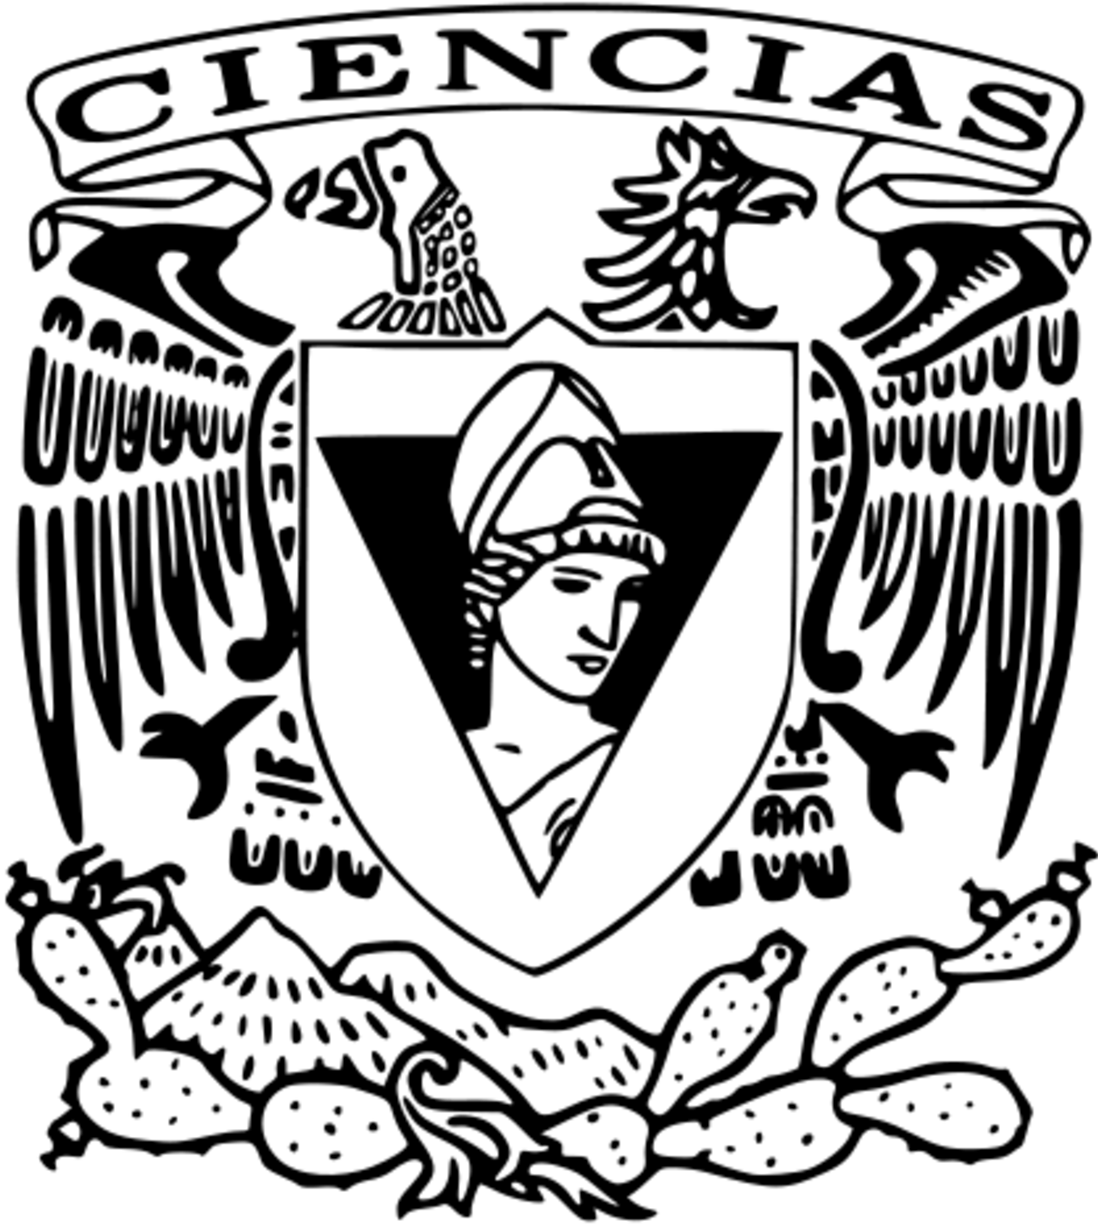
\includegraphics[height=3.4cm]{Logo_FC.png}
    	\end{center}
    \end{minipage}
\end{center}

\rule{17cm}{0.1mm}

%------ Fin de encabezado -------- %
\begin{tcolorbox}[title=Problema 1, colframe=G, coltitle=B, fonttitle=\bfseries]
\textit{Demostrar que para cualquier tri\'angulo $\Delta\,ABC$ se cumple que $\sin(A)\,\sin(B)\,\sin(C)\leq\frac{3\sqrt{3}}{8}$, ademas se tiene la igualdad si y solo si el tri\'angulo es
equilatero}  
\end{tcolorbox}
\begin{proof}
    Sea $\sin:[0,\pi]\rightarrow \R$, tenemos que la segunda derivada de $\sin$ es ella misma con signo negativo como $\sin(x)\geq 0\implies -\sin(x)\leq 0$ \\$\forall x\in [0,\pi]$, la funci\'on es concava, aplicando la desigualdad de Jenssen para $A,B,C\in [0,\pi]$\,\\
    \begin{equation*}
        \frac{1}{3}(\sin(A)+\sin(B)+\sin(C))\leq \sin\left(\frac{1}{3}(A+B+C)\right)=\sin\left(\frac{\pi}{3}\right)=\frac{\sqrt{3}}{2}
    \end{equation*}\,\\
    Luego tenemos que la funci\'on $ln:[0,\infty]\rightarrow \R$, es concava pues su derivada es $-\frac{1}{x}$, la cual es negativa para cualquier $x\in [0,\infty]$, por tanto aplicando de nuevo la desigualdad de Jenssen\,\\
    \begin{equation*}
       ln((\sin(A)\sin(B)\sin(C))^{\frac{1}{3}})=\frac{1}{3}(ln(\sin(A))+ln(\sin(B))+ln(\sin(C)))\leq ln\left(\frac{1}{3}(\sin(A)+\sin(B)+\sin(C))\right)
    \end{equation*}\,\\
    Finalmente como la funci\'on $ln$ es creciente y aplicando la primera desigualda obtenemos:\,\\
    \begin{equation*}
        ln((\sin(A)\sin(B)\sin(C))^{\frac{1}{3}})\leq ln\left(\frac{\sqrt{3}}{2}\right)
    \end{equation*}\,\\
    Finalmente exponenciando ambos lados de la desigualdad:\,\\
    \begin{equation*}
        (\sin(A)\sin(B)\sin(C))^{\frac{1}{3}}\leq \frac{\sqrt{3}}{2}\implies (\sin(A)\sin(B)\sin(C))\leq \frac{3\sqrt{3}}{8}
    \end{equation*}
\end{proof}
\begin{tcolorbox}[title=Problema 2, colframe=G, coltitle=B, fonttitle=\bfseries]
\textit{Calcular la siguiente integral:
\begin{equation*}
    \int_{0}^{1}\,\frac{x^{cos(x)}-1}{ln(x)}
\end{equation*}}  
\end{tcolorbox}
\begin{proof}\,\\
    \,\\
\end{proof}
\begin{tcolorbox}[title=Problema 3, colframe=G, coltitle=B, fonttitle=\bfseries]
\textit{Expresar el siguiente polinomio como cociente (no trivial) de dos polinomios:
\begin{equation*}
  \frac{f(x)}{g(x)}=2x+4x^3+\cdots+(2n)x^{2n-1}
\end{equation*}}  
\end{tcolorbox}
\begin{proof}
    Definimos:\,\\
    \begin{equation*}
        l(x)=x+x^2+\cdots+x^n=\frac{x^{n+1}-1}{x-1}-1=\frac{x^{n+1}-1-x+1}{x-1}=\frac{x(x^n-1)}{x-1}
    \end{equation*}\,\\
    Ademas es claro que:
    \begin{equation*}
        l(x^2)=\frac{x^2(x^{2n}-1)}{x^{2}-1}=x^2+x^4+\cdots+x^{2n}
    \end{equation*}\,\\
    Si derivamos $l(x^2)$, obtenemos:\,\\
    \begin{equation*}
        l'(x^2)(2x)=2x+4x^3+\cdots+(2n)x^{2n-1}
    \end{equation*}\,\\
    Por tanto tenemos que:\,\\
    \begin{equation*}
        \frac{(nx^{2n}(x^2-1)+1-x^{2n})(2x)}{(x-1)^2}=2x+4x^3+\cdots+(2n)x^{2n-1}
    \end{equation*}
\end{proof}
\begin{tcolorbox}[title=Problema 4, colframe=G, coltitle=B, fonttitle=\bfseries]
\textit{Si $\theta=\alpha,\beta$ son raices de la ecuaci\'on $a\cos(\theta)+b\sin(\theta)=c$, demuestra que:
\begin{equation*}
  \cos(\alpha+\beta)=\frac{a^2-b^2}{a^2+b^2}
\end{equation*}}  
\end{tcolorbox}
\begin{proof}
    Recordemos que $\sin(\theta)=\sqrt{1-\cos(\theta)}$,con $x=\cos(\theta)$ la ecuaci\'on se convierte en:\,\\
    \begin{equation*}
        ax+b\sqrt{1-x^2}=c\implies b\sqrt{1-x^2}=c-ax\implies b^2(1-x^2)=c^2-2acx+a^2x^2\implies (a^2+b^2)x^2-2acx+c^2-b^2=0
    \end{equation*}\,\\
    Finalmente obtenemos que $x=\cos(\alpha)$, $x=\cos(\beta)$ son soluciones de la siguiente ecuaci\'on cuadratica:\,\\
    \begin{equation*}
        x^2-\frac{2ac}{a^2+b^2}x+\frac{c^2-b^2}{a^2+b^2}=0
    \end{equation*}
    Por las formulas de Vieta obtenemos las siguientes relaciones:\,\\
    \begin{align*}
        \cos(\alpha)\cos(\beta)=\frac{c^2-b^2}{a^2+b^2}\,\\
        \,\\
        \cos(\alpha)+\cos(\beta)=\frac{2ac}{a^2+b^2}
    \end{align*}\,\\
    Obtendremos $sen(\alpha)\sen(\beta)$:\,\\
    \begin{equation*}
        \sin(\alpha)\sin(\beta)=\sqrt{1-\cos^2(\alpha)}\sqrt{1-\cos^2(\beta)}=\sqrt{1-(\cos^2(\alpha)+\cos^2(\beta))+\cos^2(\alpha)\cos^2(\beta)}
    \end{equation*}\,\\
    Luego obtenemos que:\,\\
    \begin{align*}
        \cos^2(\alpha)\cos^2(\beta)=\frac{(c^2-b^2)^2}{(a^2+b^2)^2}\,\\
        \,\\
        \cos^2(\alpha)+\cos^2(\beta)=\frac{4a^2c^2}{(a^2+b^2)^2}-2\frac{c^2-b^2}{(a^2+b^2)}=\frac{4a^2c^2-2(c^2-b^2)(a^2+b^2)}{(a^2+b^2)^2}
    \end{align*}\,\\
    Por tanto:\,\\
    \begin{equation*}
        \sin(\alpha)\sin(\beta)=\sqrt{\frac{(a^2+b^2)^2-(4a^2c^2-2(c^2-b^2)(a^2+b^2))+(c^2-b^2)^2}{(a^2+b^2)^2}}=\frac{\sqrt{a^4-2a^2c^2+c^4}}{a^2+b^2}=\frac{c^2-a^2}{a^2+b^2}
    \end{equation*}\,\\
    Por tanto obtenemos que:\,\\
    \begin{equation*}
        \cos(\alpha+\beta)=\cos(\alpha)\cos(\beta)-\sin(\alpha)\sin(\beta)=\frac{c^2-b^2-c^2+a^2}{a^2+b^2}=\frac{a^2-b^2}{a^2+b^2}
    \end{equation*}
\end{proof}
\begin{tcolorbox}[title=Problema 5, colframe=G, coltitle=B, fonttitle=\bfseries]
\textit{Hallar $X\in M_{3}(\R)$ tal que:
\begin{equation*}
  AXA^{T}=\begin{pmatrix}
    0 & 0 & 0 & 0\\
    0 & 2017 & 7(2017) & 2(2017)\\
    0 & 7(2017) & 49(2017) & 14(2017)\\
    0 & 2(2017) & 14(2017) & 4(2017)\\
  \end{pmatrix}\,\,\,\,con\,\,\,\,A=\begin{pmatrix}
    2 & 0 & 2\\
    0 & 1 & 0 \\
    1 & 7 & 1 \\
    7 & 2 & 7\\
\end{pmatrix}
\end{equation*}}  
\end{tcolorbox}
\begin{proof}\,\\
    \,\\
\end{proof}
\end{document}